\lhead{Background}
The problem statement is defined in the previous chapter, along with the outline of this thesis. As described in the introduction, the focal point is oversampling imbalanced data to help in classification problems. The first step is to describe popular methods when dealing with imbalanced data, before moving to the proposed model.

\section{Dealing with imbalance}
There are three popular methods for imbalanced data that will be discussed here: cost-sensitive learning, data level preprocessing methods and algorithm-level approaches. Data level preprocessing includes oversampling and undersampling. These methods handle imbalanced data during three different phases in model training. Algorithm-level approaches focus on modifying the classifier learning procedure without altering the data itself~\cite{Fernandez2018LearningSets}. The process requires an understanding of the mechanics of the classifier which lead to a bias towards the majority class. Since there are many classifiers, each with their own alterations, this topic will be limited to decision trees.

The first method depends on selecting the right algorithm and understanding its limitations in order to improve it. Decision tree classifiers are simple and efficient, and offer an interpretable solution~\cite{Safavian1991AMethodology}. A complex decision is split into a union of several smaller decisions, leading to the shape of a tree. Due to their simplicity, it is also easy to alter them from the algorithm-level approach. Each decision in the tree is made using a split function. Changing this key component is therefore the most straightforward approach possible. 

Secondly, cost-sensitive learning is also an aspect of an algorithm-level approach, but it does not alter the core algorithm itself. Instead, it introduces a missclassification cost which penalizes mistakes during classifier training. In relation with imbalanced learning this means that missclassifying the minority class is penalized during learning. The effect of imbalanced data on cost-sensitive learning has been studied~\cite{Liu2006TheStudy}, claiming that cost-sensitive classifiers still prefer a natural class distribution. In other words, highly imbalanced data needs to be balanced before applying cost-sensitive learning.

This leads to the final approach: data level preprocessing. This method involves the balancing of class distribution and can be done in three ways~\cite{Batista2004AData}
\begin{itemize}
    \item \textbf{Undersampling:} creating a subset of the original dataset by removing samples usually (from the majority class).
    \item \textbf{Oversampling:} creating a superset of the original dataset by replicating samples or creating new ones.
    \item \textbf{Hybrid methods:} Involve a combination of the undersampling and oversampling.
\end{itemize}
The simplest procedure is random undersampling and random overampling. The first method has the drawback that it potentially removes useful data. Alternatively, Random oversampling can increase the risk of oversampling, as the method makes exact copies of existing samples~\cite{Fernandez2018LearningSets}. Both undersampling and oversampling have been studied and many methods have been proposed. This thesis focuses on oversampling, specifically SMOTE-based oversamplers.

\section{SMOTE algorithm}
SMOTE is an acronym for Synthetic Minority Oversampling TEchnique. The method was first introduced by Chawla et al.~\cite{Chawla2002SMOTE:Technique} in 2002. The main idea is to introduce new, synthetic samples to the dataset to make it balanced. These samples are created by interpolation between samples of the minority class. 

\begin{figure}
    \centering
    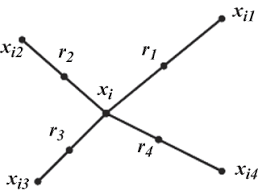
\includegraphics[width=.4\textwidth]{Thesis/Figures/SMOTE_alg.png}
    \caption{An illustration of how to create synthetic data samples using the SMOTE algorithm~\cite{Fernandez2018LearningSets}.}
    \label{fig:SMOTE}
\end{figure}

An example of the SMOTE algorithm works is given in figure~\ref{fig:SMOTE}. First, a sample $x_i$ is taken from the minority class. Then, using a distance metric (ie. Euclidian distance), $k$ nearest neighbours are selected, points $x_{i1}$ to $x_{i4}$. Finally, these points are randomly interpolated to create new instances labelled as $r_1$ to $r_4$. This process is repeated until the desired ratio between majority and minority class is achieved. 

\section{SMOTE extensions}
SMOTE is now widely known and easy to implement in Python, due to its inclusion in the Imbalanced-learn package~\cite{Lemaitre2017Imbalanced-learn:Learning}. Since 2002, many variations of SMOTE were introduced, changing parts of the algorithm to improve its performance in classification. Sometimes these changes allow for more use. SMOTE relies on a nearest neighbour algorithm, which is difficult to define for categorical features. In Chawla et al.'s original SMOTE article, SMOTE-NC was also introduced~\cite{Chawla2002SMOTE:Technique}. The NC is short for Nominal Continuous, and alters the distance metric to account for nominal features. Consider two features with both numerical and nominal samples
\begin{align}
    F_1 = [1,2,3,A,B,C]  \\
    F_2 = [5,6,7,A,D,E]
\end{align}
For the continuous features, the Euclidian distance can be easily calculated. If the nominal features differ between samples, then the median of standard deviations of all continuous features for the minority class is included. In the case of our two features, the Euclidian distance is calculated as
\begin{align}
    d_{Eucl} = \sqrt{[(5-1)^2 + (6-2)^2 + (7-3)^2 + Med^2 + Med^2]}
\end{align}
The synthetic samples are then generated similarly to SMOTE.

Another example is Borderline-SMOTE, which synthesizes minority samples near the decision boundary~\cite{Han2005Borderline-SMOTE:Learning}. This algorithm also considers the majority samples surrounding a minority sample. If a minority sample is surrounded by more majority samples than minority samples, it is marked as easily missclasified and added to a special set $D$. Once all minority samples are considered, the samples from $D$ are then oversampled in the same way as in regular SMOTE.

Another SMOTE-based oversampler is ADASYN, an acronym for ADAptive SYNthetic sampling approach~\cite{He2008ADASYN:Learning}. ADASYN introduces a new learning constraint, where it uses the weighted distribution for different minority samples according to their difficulty in learning. More samples will be synthesized for samples that are harder to learn. Similar to Borderline-SMOTE, a sample surrounded by majority samples is considered harder to learn. However, ADASYN uses a density distribution for all minority samples to decide where to synthesize new samples.

\begin{figure}
  \begin{subfigure}[t]{.4\textwidth}
    \centering
    \includegraphics[width=\linewidth]{example-image-a}
    \caption{\textbf{Schnitt}: $A \cup B$: Element liegt in $A$ \textbf{oder} in $B$.}
  \end{subfigure}
  \hfill
  \begin{subfigure}[t]{.4\textwidth}
    \centering
    \includegraphics[width=\linewidth]{example-image-b}
    \caption{\textbf{Vereinigung}: $A \cap B$: Element liegt in $A$ \textbf{und} in $B$.}
  \end{subfigure}

  \medskip

  \begin{subfigure}[t]{.4\textwidth}
    \centering
    \includegraphics[width=\linewidth]{example-image-c}
    \caption{\textbf{Differenz}: $A \setminus B$: Element liegt in $A$ \textbf{nicht} in $B$. (\textit{A ohne B})}
  \end{subfigure}
  \hfill
  \begin{subfigure}[t]{.4\textwidth}
    \centering
    \includegraphics[width=\linewidth]{example-image-a}
    \caption{\textbf{Symmetrische Differenz}: $A \Delta B$: Element liegt \textbf{entweder} in $A$ oder in $B$.}
  \end{subfigure}
\end{figure}

Small bit about comparison figure SMOTE